%==============================================================================
% Sjabloon poster bachproef
%==============================================================================
% Gebaseerd op document class `a0poster' door Gerlinde Kettl en Matthias Weiser
% Aangepast voor gebruik aan HOGENT door Jens Buysse en Bert Van Vreckem

\documentclass[a0,portrait]{hogent-poster}

% Info over de opleiding
\course{Bachelorproef}
\studyprogramme{toegepaste informatica}
\academicyear{2025-2026}
\institution{Hogeschool Gent, Valentin Vaerwyckweg 1, 9000 Gent}

% Info over de bachelorproef
\title{Hoe kan een end-to-end monitoringoplossing IT-incidenten tijdig detecteren binnen het havenlandschap?}
\author{Milan De Caigny}
\email{milan.decaigny@student.hogent.be}
\supervisor{Veerle Depestele}
\cosupervisor{Frederik Baert (Sea-Invest)}

% Indien ingevuld, wordt deze informatie toegevoegd aan het einde van de
% abstract. Zet in commentaar als je dit niet wilt.
\specialisation{Systeem- en Netwerkbeheer}
\keywords{End-to-end monitoring, traditionele monitoring, Checkmk, Robotmk, IT-incidenten}
\projectrepo{https://github.com/MilanDeCaigny/Bachelorproef-25-26-MDC}

\begin{document}

\maketitle

\begin{abstract}
Traditionele monitoring detecteert voornamelijk infrastructuurproblemen, terwijl end-to-end monitoring inzicht biedt in applicatiefouten en gebruikersflows. In deze bachelorproef werd een proof-of-concept ontwikkeld met Checkmk en Robotmk om beide monitoringmethoden te vergelijken.
\end{abstract}

\begin{multicols}{2}
    
    \section{Probleemstelling}
    
  Traditionele monitoring controleert vooral servers, services en infrastructuur. Problemen binnen applicaties of gebruikersflows blijven hierdoor niet altijd zichtbaar.
    
    \section{Onderzoeksvraag}
    
  Hoe kan een end-to-end monitoringoplossing worden ontworpen en geïmplementeerd om IT-incidenten tijdig te detecteren en sneller op te lossen binnen het havenlandschap?
    
    \section{Methodologie}
    
    \begin{center}
    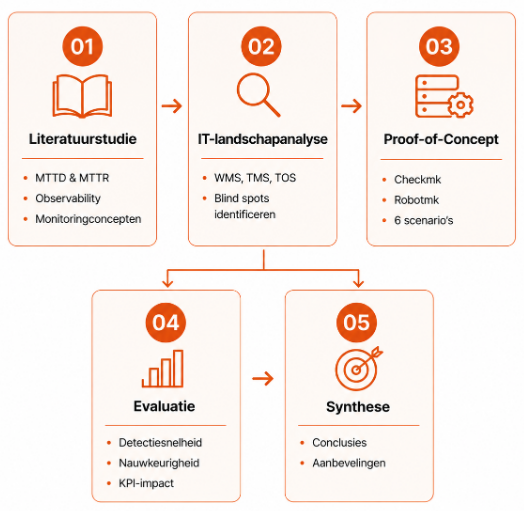
\includegraphics[width=0.9\linewidth]{methodologie}
    \end{center}
    
    \section{Proof-of-Concept}
    
    \begin{center}
        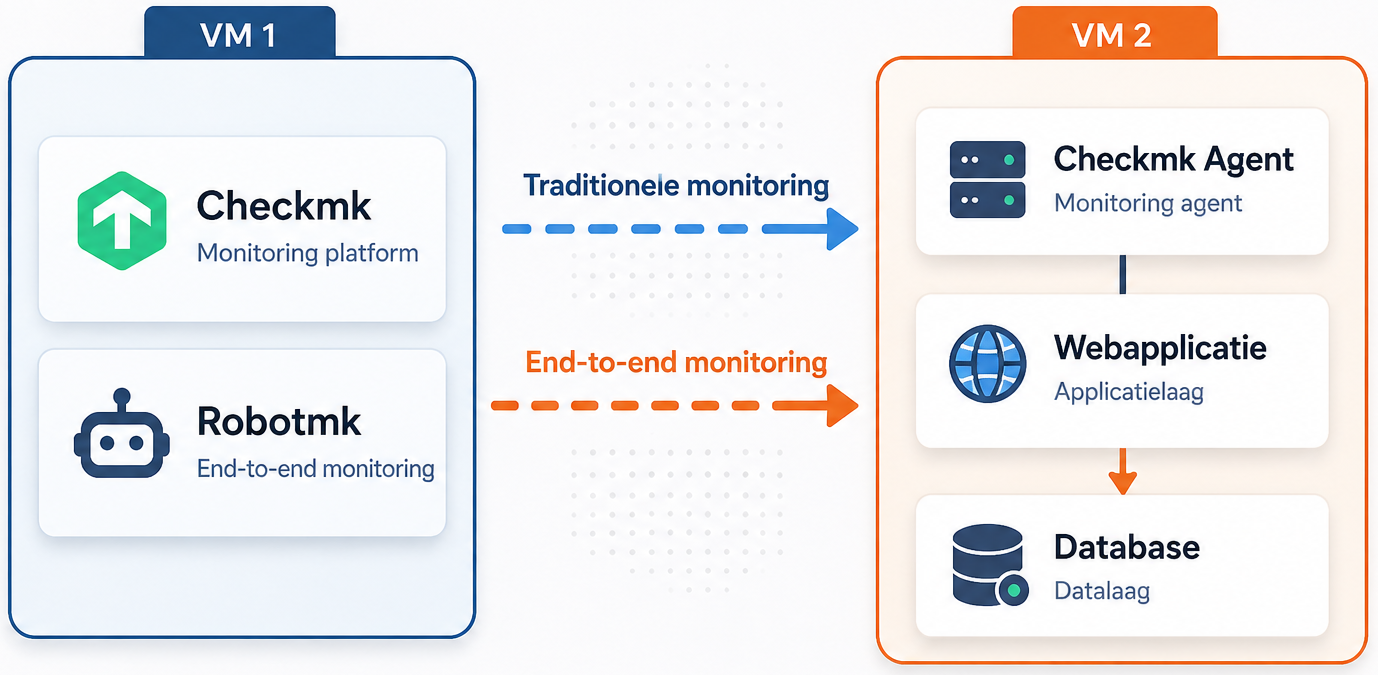
\includegraphics[width=1.0\linewidth]{architectuur2}
        \vspace{0.2cm}
        {\small \textbf{Figuur 1:} Opbouw van de proof-of-concept omgeving}
    \end{center}
    
    \columnbreak
    \section{Monitoringresultaten}
    
    \begin{center}
        {\color{orange}\Large\textbf{Traditionele monitoring}}\\[0.1cm]
        {\color{orange}\normalsize(Infrastructuur \& services)}\\[0.3cm]
        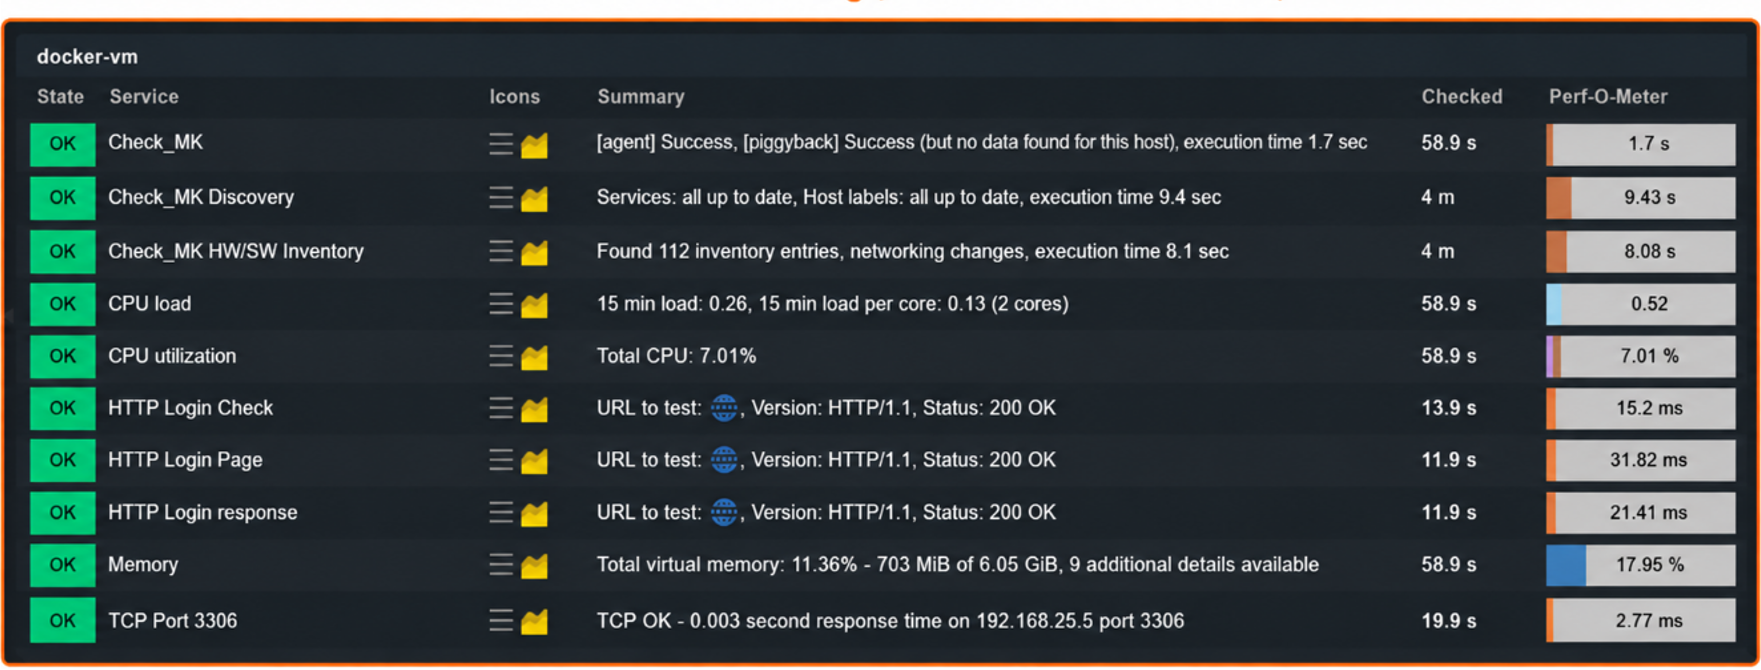
\includegraphics[width=1.1\linewidth]{Checkmk-Resultaten}
        \vspace{0.2cm}
        {\small \textbf{Figuur 2:} Overzicht van traditionele monitoringchecks in Checkmk}
        
        {\color{cyan}\Large\textbf{End-to-end monitoring}}\\[0.1cm]
        {\color{cyan}\normalsize(Gebruikersflows \& applicatietesten)}\\[0.3cm]
        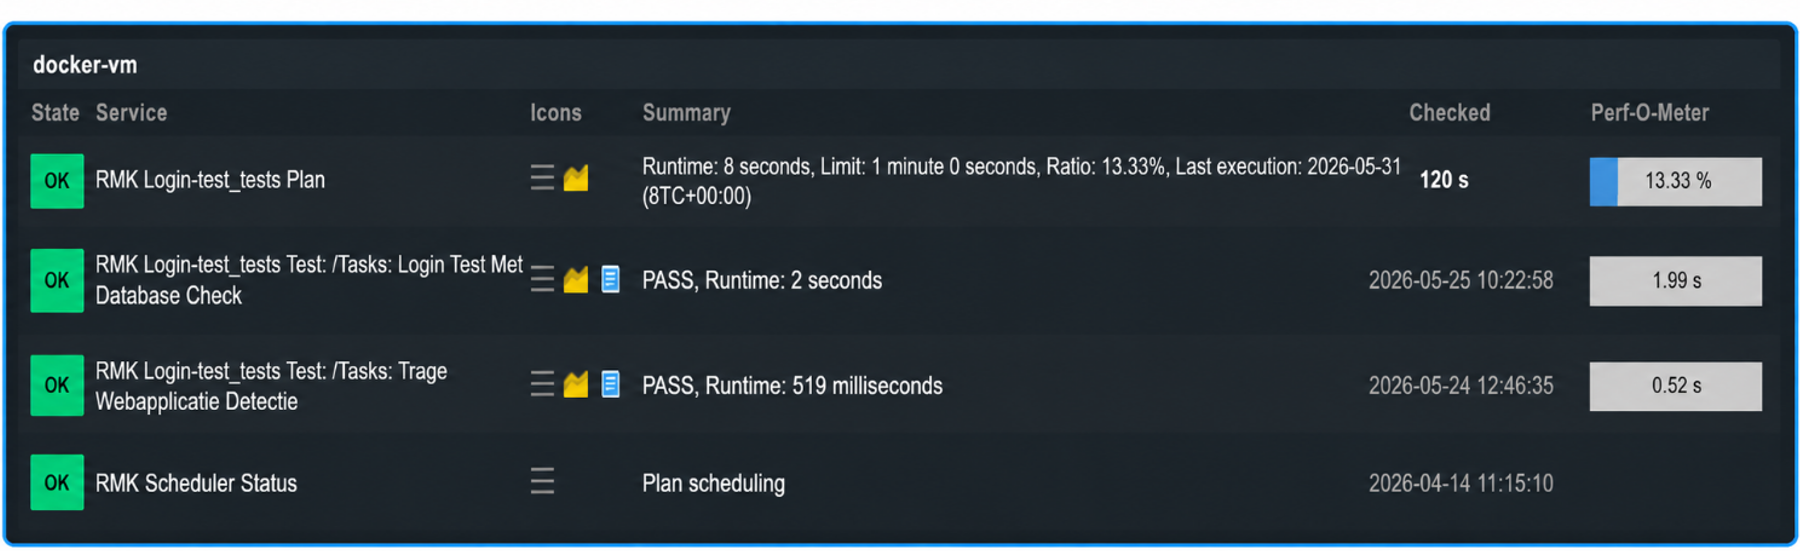
\includegraphics[width=1.1\linewidth]{Robotmk-Resultaten}
        \vspace{0.2cm}
        {\small \textbf{Figuur 3:} Overzicht van end-to-end monitoringchecks in Checkmk}
    \end{center}
    
    \section{Resultaten}
    
    \begin{center}
        \includegraphics[width=1.1\linewidth]{Resultaten}
    \end{center}
    
    \section{Conclusie}
    
    \begin{itemize}
        \item Traditionele monitoring detecteert infrastructuurproblemen.
        \item End-to-end monitoring detecteert applicatie- en gebruikersproblemen.
        \item Een combinatie van beide monitoringmethoden biedt de grootste meerwaarde.
    \end{itemize}
    
\end{multicols}
\end{document}